\documentclass[12pt,a4paper]{article}
\usepackage{amsmath}
\usepackage{amsfonts}
\usepackage{amssymb}
\usepackage{graphicx}
\usepackage{secdot}
\usepackage[left=2cm,right=2cm,top=2cm,bottom=2cm]{geometry}

\author{Shibayan Biswas, AE21B109\\ Department of Aerospace Engineering\\ IIT Madras}

\title{Assignment - 1}

\date{August 24, 2022}

\begin{document}

\maketitle
\hline
\section{Introduction:}
In this assignment the task given to us was to create a well-labelled two-dimensional plot using Python 3 that describes a function of our choice and to create a three-dimensional plot using Octave of a function of our choice.
\section{Two-dimensional plot using Python 3:}
In this section I have plotted the two-dimensional plot using Python 3 for the function of my choice, The function of my choice is the Exponential function which is represented below by the given equation:
\begin{equation}
    \text{f}(x) = \text{$e^x$}
\end{equation}
The plot of the above function using Python 3 is shown below:
\begin{figure}[!ht]
	\begin{center}
		\framebox{
			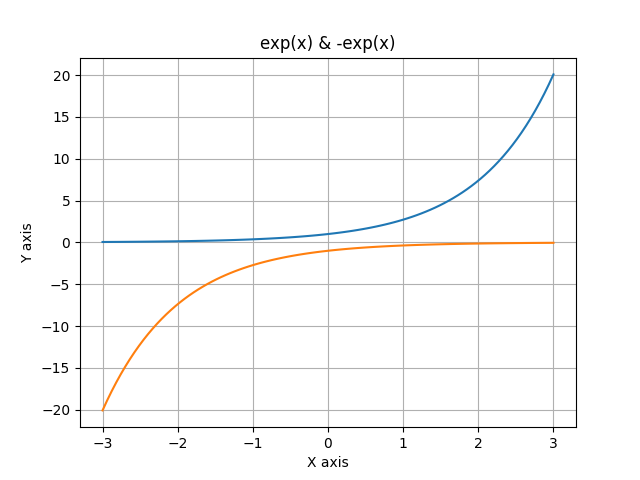
\includegraphics[scale=0.7]{Figure_1.png}
		}
	\end{center}
	\caption{Two-dimensional plot of f(x) = $e^x$ using Python 3}
\end{figure}
\section{Three-dimensional plot using Octave:}
In this section I have plotted the three-dimensional plot using Octave for the function of my choice, The function of my choice is the Logarithmic function which is represented below by the given equation:
\begin{equation}
    \text{f}(x) = \text{ln}(x)
\end{equation}
The plot of the above function using Python 3 is shown below:
\begin{figure}[!ht]
	\begin{center}
			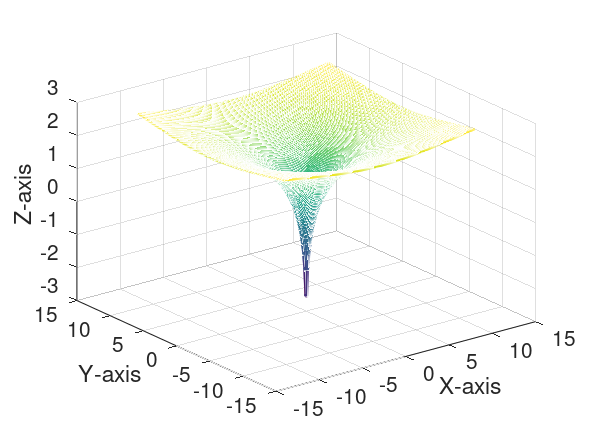
\includegraphics[scale=0.8]{Figure_2.png}
	\end{center}
	\caption{Three-dimensional plot of f(x) = ln(x) using Octave}
\end{figure}
\section{Conclusion:}
In this particular project I have created a well-labelled two-dimensional plot using Python 3 that describes a function of my choice and a three-dimensional plot using Octave of a function of my choice. In this section I will providing a brief introduction about the functions whose graphs I have plotted. This is represented below:
\subsection{Exponential Function ($e^x$) :}
The exponential function is a mathematical function denoted by f(x) = exp(x) or $e^x$ (where the argument x is written as an exponent). Unless otherwise specified, the term generally refers to the positive-valued function of a real variable, although it can be extended to the complex numbers or generalized to other mathematical objects like matrices or Lie algebras. The exponential function originated from the notion of exponentiation (repeated multiplication), but modern definitions (there are several equivalent characterizations) allow it to be rigorously extended to all real arguments, including irrational numbers. Its ubiquitous occurrence in pure and applied mathematics led mathematician Walter Rudin to opine that the exponential function is "the most important function in mathematics".
\subsection{Logarithmic Function ($ln(x)$) :}
In mathematics, the logarithm is the inverse function to exponentiation. That means the logarithm of a given number x is the exponent to which another fixed number, the base b, must be raised, to produce that number x. In the simplest case, the logarithm counts the number of occurrences of the same factor in repeated multiplication. The logarithm of x to base b is denoted as $log_b$(x), or without parentheses, $log_b x$, or even without the explicit base, $log x$, when no confusion is possible, or when the base does not matter such as.
\end{document}
